\documentclass{article}

\usepackage{tikz}
\usetikzlibrary{angles,quotes}
\begin{document}

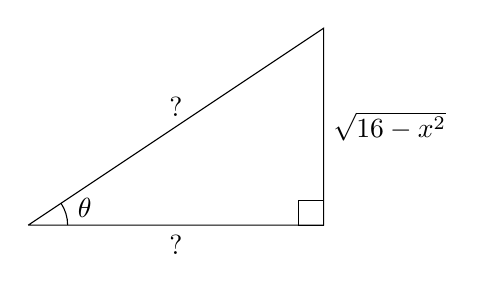
\begin{tikzpicture}[scale=1.25]%,cap=round,>=latex]
\coordinate [] (A) at (-1.5cm,-1.cm);
\coordinate [] (C) at (1.5cm,-1.0cm);
\coordinate [] (B) at (1.5cm,1.0cm);
\draw (A) -- node[above] {$?$} (B) -- node[right] {$\sqrt{16-x^2}$} (C) -- node[below] {$?$} (A);

\draw (1.25cm,-1.0cm) rectangle (1.5cm,-0.75cm);
\pic [draw, "$\theta$", angle eccentricity=1.5] {angle = C--A--B};

\end{tikzpicture}

\end{document}
